
\begin{figure}
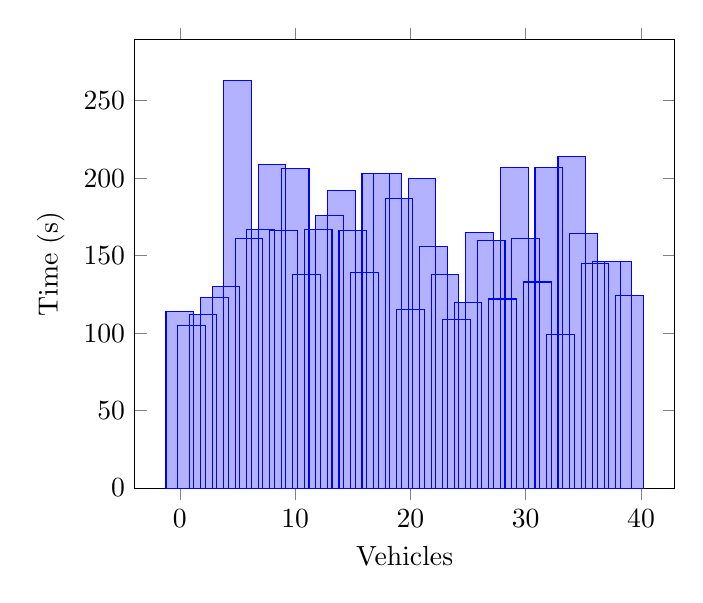
\begin{tikzpicture}
\begin{axis}[
legend style={anchor=west},
xlabel=Vehicles,
ylabel=Time (s),
ymin=0,
ybar,
]
\addplot coordinates {
(0, 114)
(1, 105)
(2, 112)
(3, 123)
(4, 130)
(5, 263)
(6, 161)
(7, 167)
(8, 209)
(9, 166)
(10, 206)
(11, 138)
(12, 167)
(13, 176)
(14, 192)
(15, 166)
(16, 139)
(17, 203)
(18, 203)
(19, 187)
(20, 115)
(21, 200)
(22, 156)
(23, 138)
(24, 109)
(25, 120)
(26, 165)
(27, 160)
(28, 122)
(29, 207)
(30, 161)
(31, 133)
(32, 207)
(33, 99)
(34, 214)
(35, 164)
(36, 145)
(37, 146)
(38, 146)
(39, 124)
};

\end{axis}
\end{tikzpicture}
\label{tik:100:1_S, 1_S.-60, 4_S, 5_S, 5_S.-30, 7_S, 7_S.-25, 11_S, 11_S.-50, 13_S, 15_N, 17_S, 17_S.-60, 19_V}
\caption{100 percent diving with GSC on route $1_S, 1_S.-60, 4_S, 5_S, 5_S.-30, 7_S, 7_S.-25, 11_S, 11_S.-50, 13_S, 15_N, 17_S, 17_S.-60, 19_V$}
\end{figure}
